\documentclass[]{IEEEtran}
\usepackage{epsfig}
\usepackage{subfigure}

%\textwidth 7.5in% \textheight 23.0cm
%\oddsidemargin -0.5in
%\evensidemargin -0.5in
%%%%%\topmargin -0.5in
%\parskip 0.25ex
%\parindent 1.5ex
%\sloppy
%\raggedbottom


\def \ie {{\it i.e.}, }
\def \eg {{\it e.g.}, }

\newcommand{\tile}{tile}
\newcommand{\Tile}{Tile}
\newcommand{\tiles}{tiles}
\newcommand{\Tiles}{Tiles}
\newcommand{\ntiles}{16}

%\newlength{\itemhack}
%\setlength{\itemhack}{-0.088in}

%\newlength{\parhack}
%\setlength{\parhack}{-0.12in}


\begin{document}
\title{StreamIt: A Language and Compiler for Communication-Exposed Architectures}

%\numberofauthors{1}
%\author{
%\alignauthor \vspace{-28pt}
%William Thies, 
%Michael Gordon, 
%Michal Karczmarek, 
%David Maze, 
%and Saman Amarasinghe\\
%	\vspace{6pt}
%	{\large \{thies, mgordon, karczma, dmaze,
%	saman\}@lcs.mit.edu} \\ 
%	\vspace{6pt}
%	Laboratory for Computer Science, Massachusetts Institute of
%	Technology\\ \vspace{-12pt}
%%	\vspace{12pt}
%%        \today
%}

\author{\authorblockN{{\large William Thies, Michael I. Gordon, Michal Karczamarek, \\ 
David Maze, and Saman Amarasinghe\\}}
\authorblockA{\{thies, mgordon, karczma, dmaze, saman\}@lcs.mit.edu\\
Laboratory for Computer Science, Massachusetts Institute of Technology}}

\maketitle

\begin{abstract}
Due to the high data rates involved in audio, video, and signal
processing applications, it is imperative to compress the data to
decrease the amount of storage used.  Unfortunately, this implies that
any program operating on the data needs to be wrapped by a
decompression and re-compression stage.  Re-compression can incur
significant computational overhead, while decompression swamps the
application with the original volume of data.

In this paper, we present a program transformation that greatly
accelerates the processing of compressible data.  Given a program that
operates on uncompressed data, we output an equivalent program that
operates directly on the compressed format.  Our transformation
applies to stream programs, a restricted but useful class of
applications with regular communication and computation patterns.  Our
formulation is based on LZ77, a lossless compression algorithm
utilized by ZIP, and immediately applies to simpler formats such as
Apple Animation, Microsoft RLE, and Targa.

We implemented a simple subset of our techniques in the StreamIt
compiler, which emits executable plugins for two popular video editing
tools: MEncoder and Blender.  For common operations such as color
adjustment and video compositing, computing directly on compressed
data offers a speedup roughly proportional to the overall compression
ratio.  For our benchmark suite of 12 videos in Apple Animation
format, speedups range from 1.1x to 471x, with a median of 15x.

\end{abstract}

\setcounter{bottomnumber}{5}
\setcounter{topnumber}{5}
\setcounter{dbltopnumber}{2}

\section{Introduction}


Stream computing represents an increasingly important class of
applications. In streaming codes, there is an abundance of parallelism that
is easier to extract compared to traditional desktop workloads (e.g.,
pointer-based computing). As a result, the extraction of parallelism
in streaming codes does not require heroic efforts, and thus,
processors can deliver higher performance with significantly lower
power costs. This is especially important since
leading microprocessor companies have realized that modern general
purpose architectures are near their  performance limits for  the
amount of power they consume. Thus, the future will place a greater
emphasis on exploiting the properties of streaming workloads in
conventional von~Neumann architectures.

Streaming is a model of computation that uses sequences of data
and computation kernels to expose concurrency and locality for
efficiency~\cite{wss}. In general purpose processors, improving locality 
translates to an effective management of the memory hierarchy at all
levels, including the register file. In this paper, we present a
methodology for compiling streaming codes to general purpose,
cache-based architectures. We first introduce a simple model for
reasoning effectively about the caching behavior of streaming
workloads. This model serves as a foundation for several {\it cache-aware
optimizations} that are geared toward the concomitant increase of instruction
and data {\it temporal locality}. These
optimization lead to significantly better utilization of the memory
system, and as such, they deliver performance gains ranging from 11
to 99\% for our streaming benchmark suite.

The context for our work is StreamIt, an architecture-independent
language that is engineered for streaming
applications~\cite{streamitcc}. It adopts the 
Cyclo-Static Dataflow~\cite{BELP96} model of computation which is a
generalization of Synchronous Dataflow~\cite{LM87-i} (SDF).  
SDF is a popular  model that  is well suited for
streaming codes. In SDF, computation is represented as a graph
consisting of {\it  actors} connected by communication channels; the
actors consume  and produce a constant number  of items from their
input and output  channels every time they execute. SDF is appealing
because it is amenable to static scheduling and optimization. 

From a general purpose architecture's point of view, actors represent
computation kernels, and the communication between actors represents
data buffers that must be streamed to and from the processor. Thus
the size of an actor and the
order of actor executions are critical properties that
impact the performance of the instruction cache. For example, the
compiler must make sure the actor's code size is not
greater than the instruction cache. Furthermore, we must {\it scale}
the execution of the actor so that it runs several times before we move
on to some other actor in the stream 
graph. This serves to $(i)$ amortize the cost of fetching the actor's
instructions into the cache from memory (an expensive operation), $(ii)$
improve the instruction temporal locality, and $(iii)$ improve overall
performance. However, as our cache model will show, we 
cannot arbitrarily scale the execution frequency of an actor. This
is because actors produce data that must be buffered, and therefore,
we must also consider the amount of data an actor produces and
consumes if we are to adequately manage the data cache. This paper is unique
in that it is the first to present a unified optimization methodology
that simultaneously considers instruction and data locality for
mapping streaming computation to cache-based architectures.

In terms of improving the data cache behavior, the compiler schedules
actor firing such that the producer-consumer locality is
preserved. Furthermore,  the compiler may {\it fuse}
together two or more actors to form a coarser grained kernel.
The fusion allows for better register allocation as we can
destroy the arrays used to buffer data between the actors and replace
the corresponding array references with scalars.  It also allows for
various competing implementations for managing the buffers between the
fused actors.  This paper evaluates several implementation
alternatives (for buffer management) and evaluates their performance.

The methodology for fusing actors leverages a distinguishing StreamIt
characteristic, namely, the hierarchical organization of
the stream graph. Furthermore, the algorithm for fusing actors applies
for the various topologies allowed by StreamIt.
It also considers another distinguishing characteristics of StreamIt,
namely the {\tt peek} operation whereby an actor may inspect data
items in its input buffer without consuming them until some future
execution. While peeking is a powerful language feature, it does pose
some challenges to the compiler and the cache optimizations. Peeking
also impacts the choice for the best buffer management strategy, as our
study will show.

%% the comment about p3 and itanium not being embedded architectures
%% is out of the blue! need a better transition.
Cache-aware fusion alone delivers significant performance gains, although our
evaluation shows that fusion with scaling leads to the best
performance on a general purpose, cache-based architecture. For our
experiments, we use two different processors: a superscalar out-of-order
processor, and an in-order VLIW processor. The former is a Pentium~3
whereas the latter is an Itanium~2. While these architectures are not
particularly suited for an embedded system, they do exhibit some
properties that are worthy of investigation. Furthermore, that we can
demonstrate measurable performance gains on real systems is far more
convincing than using a simulation-based environment. We chose the
Pentium~3 processor because it has very few registers in its
instruction set architecture. The Itanium by contrast has a much 
larger and richer repertoire of registers. The two architectures serve
to validate our cache-aware optimizations, in that we expect an
architecture with more register to benefit more from optimization such
as scalar replacement. On average, fusion leads to a 47\% improvement
on the Pentium~3, and 50\% on the Itanium~2.

The two architectures also differ in terms of their memory system
organization. The Itanium is an in-order VLIW processor and does not
tolerate a memory stall as well as its out-of-order
counterpart. Therefore we expect different gains from the scaling
optimization which amortize the long access latencies for instruction
and data caches. On average, scaling leads to a 21\% improvement on
the Itanium~2, and 17\% on the Pentium~3.

While both scaling and fusion lead to modest performance gains, we
must combine the two to deliver the best possible performance. When we
do so, we can further improve the performance of our benchmarks by
53\% on average for the Pentium~3, and 55\% for the Itanium~2.

\subsection{Summary of Contributions}

This paper makes the following contributions:
\begin{itemize}

\item A cache model for stream computing that provides a quantitative
estimate of the caching performance for any sequence of actor
executions.

\item A cache-aware scheduling heuristic that judiciously increases
the multiplicity of actors, improving instruction and data locality
while not exceeding the data cache.

\item A cache-aware partitioning policy that judiciously fuses
adjacent actors into a single component, enabling local optimizations
while not exceeding the instruction cache.

\item An optimized buffer management policy, termed ``copy-shift with
execution scaling'', which out-performs a traditional rotating buffer
in a detailed micro-benchmark analysis.

\item A fully automatic implementation of the above techniques in the
StreamIt compiler.

\item An experimental evaluation across 11 streaming benchmarks,
demonstrating performance improvements of up to 99\%.
\end{itemize}

\subsection{Paper Roadmap}

The remainder of the paper is organized as follows. Section~\ref{sec:streamit}
describes StreamIt and introduces our motivating example.
Section~\ref{sec:cache-model} introduces our cache model for 
reasoning about the performance of a streaming
computation. Section~\ref{sec:cache-opt} describes our cache-aware
optimizations, and Section~\ref{sec:buffer} describes the 
optimization enabled by fusion. Section~\ref{sec:evaluation} describes
our evaluation methodology and present our experimental
analysis. Sections~\ref{sec:related-work}~and~\ref{sec:conclusion}
discuss related work and concludes the paper.

\section{StreamIt}
\label{sec:streamit}

StreamIt  is   an  architecture-independent  language that was
designed for  streaming applications. In StreamIt, programs are
represented as graphs where  nodes represent  computation and edges
represent FIFO-ordered communication of data over tapes.

The  basic programmable  unit (i.e., an actor) in  StreamIt is a {\it
filter}.   Each filter contains  a work  function that executes
atomically,  popping (i.e., reading)  a fixed number  of items  from
the  filter's input  tape and pushing (i.e., writing) a fixed number
of items to the filter's output tape.  A filter  may also {\tt peek} at
a given index  on its input tape without  consuming  the  item;  this
makes  it  simple  to  represent computation over a
sliding-window.   The {\tt push}, {\tt pop}, and {\tt peek} rates are
declared as part  of  the work  function,  thereby enabling  the
compiler    to construct a static schedule of filter executions. The
following is an example implementation of a FIR   (Finite Impulse
Response)  filter: 
%\begin{scriptsize}
{\small
\begin{verbatim}
float->float filter FIR (int N, float[] weights) 
{
  work push 1 pop 1 peek N {
    float sum = 0;
    for (int i = 0; i < N; i++) {
      sum += peek(i) * weights[i];
    }
    pop();
    push(sum);
  }
}
\end{verbatim}}
%\end{scriptsize}

The work function is invoked (fired) whenever there is sufficient data
on the input tape. In this case, the filter requires at least
\texttt{N} elements before it can execute. The value of \texttt{N} is
known at compile time when the filter is composed to form a stream
graph. A filter is akin to a class in object oriented programming
with the work function serving as the main method. The parameters
to a filter (e.g., \texttt{N} and \texttt{weights}) are equivalent to
parameters passed to a class constructor. In StreamIt, the
application developer focuses on the hierarchical assembly of the
stream graph and its communication topology, rather than on the 
explicit management of the data buffers between filters.

\begin{figure}[t]
\begin{center}
\vspace{-24pt}
 \framebox{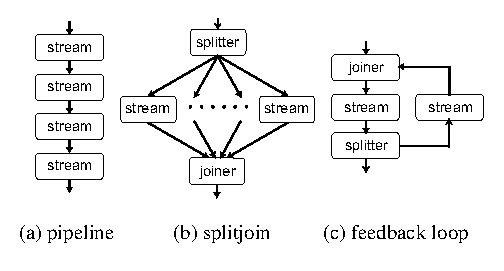
\includegraphics[scale=1, angle=0]{./constructs-eg.eps}}
 \vspace{-6pt}
 \caption{StreamIt containers.}
 \label{fig:containers}
\end{center}
\end{figure}

\begin{figure}[t]
\begin{center}
\vspace{-12pt}
 \framebox{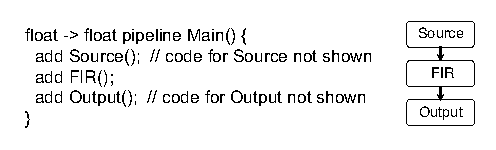
\includegraphics[scale=1, angle=0]{./pipeline-eg.eps}}
 \vspace{-6pt}
 \caption{Example pipeline with FIR filter.}
 \label{fig:pipeline}
\vspace{-18pt}
\end{center}
\end{figure}

StreamIt provides three hierarchical structures for composing filters
into larger stream graphs (see Figure~\ref{fig:containers}). The 
{\it pipeline} construct composes streams in sequence, with the output
of one connected to the input of the next.   An example of a pipeline
appears in Figure~\ref{fig:pipeline}.

The {\it splitjoin} construct distributes data to a set of parallel
streams, which are then joined together in a round robin fashion.  In
a splitjoin, the {\it splitter} performs the data scattering, and the
{\it joiner} performs the gathering. A splitter is a specialized
filter with a single input and  multiple output channels. On 
every execution step, it can distribute its output to any one of
its children in either a {\it duplicate} or a {\it roundrobin}
manner. For the former, incoming data is replicated to every
sibling connected to the splitter. For the latter, data is scattered
in a round-robin manner, with each item sent to exactly one child
stream, in order.  The splitter type and the weights for distributing data to
child streams are declared as part of the syntax (e.g., \texttt{split
duplicate} or \texttt{split roundrobin($w_0$, $w_1$, ... $w_n$)}). The
splitter counterpart, the joiner, is a specialized filter with  
multiple input channels but only one output channel. The joiner
gathers data from its predecessors in a round-robin manner (declared
as part of the syntax). 

StreamIt also provides a {\it feedback loop} construct for introducing
cycles in the graph.

\section{Execution Model}
\label{sec:execmodel}

A StreamIt program is represented by a hierarchical graph,
where the leaf nodes are filters, splitters, and joiners, and
the composite nodes are pipelines, splitjoins, and
feedback-loops. Edges in the graph represent data channels, which 
operate as FIFO queues.
In order for an actor  (i.e., a filter,
splitter, or joiner) to execute, it must have enough data items on its input
tape. In StreamIt, actors have  two epochs
of execution: one for initialization, and one for the steady
state. The initialization primes the input tapes to allow filters with
peeking to execute the very first instance of their work functions;
initialization in this setting is similar to the prologue stage in
software pipelining. The steady state schedule has the property that
the amount of data buffered between any two actors does not change
before and after the actor executions.

\begin{figure}[t]
\begin{center}
\vspace{-24pt}
 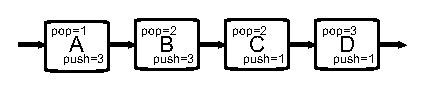
\includegraphics[scale=1, angle=0]{./pipe-with-rates.eps}
\vspace{-6pt}
 \caption{Example pipeline.}
 \label{fig:pipe-with-rates}
\end{center}
\end{figure}

As an example, a steady state schedule for the sample pipeline in
Figure~\ref{fig:pipe-with-rates} requires filter \texttt{A} to fire
four times, \texttt{B} six times, \texttt{C} nine times, and
\texttt{D} three times. 
% Because in StreamIt the filters are
% independent (i.e., they do not share state), they can execute
% concurently. In a uniprocessor setting (which is what we use for our
% evaluation), we can only run one filter at time. Therefore, 
The data generated by one actor is buffered (cached) until it is
consumed.

The StreamIt compiler derives the initialization and steady state
schedules~\cite{karczma-lctes03} and outputs a C program that includes
the initialization and work functions, as well as a driver to execute
each of the two schedules. For example, referring to
Figure~\ref{fig:pipe-with-rates}, the compiler generates the following
sample code for running the steady state schedule:
%\begin{scriptsize}
\begin{verbatim}
run_steady_state() {
  for (i = 0; i < 4; i++) A_work();
  for (i = 0; i < 6; i++) B_work();
  for (i = 0; i < 9; i++) C_work();
  for (i = 0; i < 3; i++) D_work();
}
\end{verbatim}
%\end{scriptsize}
To execute the program, the steady state kernel is wrapped with
another loop that invokes the kernel a designated number of
times. Preceding the state steady, a similar initialization schedule
is run to prime the data buffers, and following the steady state, an
epilogue is run to drain the buffers as necessary.

\begin{figure}[t]
\begin{center}
\vspace{-12pt}
 \psfig{figure=ssi.eps,width=3in}
 \vspace{-6pt}
 \caption{Instruction size (in bytes along the y-axis) per filter
 (x-axis) occurring in a steady state execution of FFT.}
 \label{fig:ssi-single}
\vspace{-18pt}
\end{center}
\end{figure}

From a caching point of view, it is intuitively clear that once a
filter's instruction working set is fetched into the cache, we must
execute that filter as many times as possible to improve instruction
locality and amortize the cost of the accesses to lower levels of the
memory hierarchy. This of course assumes that the total code size for
the filters in the steady state exceeds the capacity of the
instruction cache (which is commonly the case;). In
Figure~\ref{fig:ssi-single} we show a representative breakdown of the
code size per filter in a steady state execution of a StreamIt
implementation of FFT. In all, the total code size for a steady state
ranges from 16~Kb to over 60~Kb for our benchmarks. These results
provide evidence that while individual filters may have a
small instruction footprint, the total footprint of the filters in a
steady state exceeds a typical instruction cache size.
From these observations, it is evident that we must {\it scale} the
execution of filters in the steady state in order to improve temporal
locality. In other words, rather than running a filter $S$ times per
steady state, we increase the loop bound so that it runs $\texttt{M}
\times S$ times (e.g., the loop bound for \verb+A_work+ is
changed to $\texttt{M} \times 4$ in the example shown earlier). 
We term \texttt{M} the {\it multiplicity factor}.

The obvious question is: to what extent can we scale the execution of
filters in the steady state? The answer is non-trivial because
scaling, while beneficial to the instruction cache behavior, may
overburden the data cache as the buffers between actors may grow to
prohibitively large sizes that degrade the data cache
behavior. Specifically, if a buffer overflows the cache, then
produce-consumer locality is lost. 

Also complicating matters is the amount of state a filter must retain
from one execution of its work function to the next. In the FIR
example shown earlier, the filter state is proportional to the size of
the coefficient array (i.e., \texttt{weights}). The filter state
further constrains the schedule scaling.

\section{Compiling StreamIt to Raw}
\label{sec:phases}
StreamIt language aims to be portable across communication-exposed
machines.  StreamIt expose the parallelism and communication of
streaming applications without depending on the topology or
granularity of the underlying architecture.  have implemented a
fully-functional prototype of the StreamIt compiler for
Raw~\cite{raw}, a tiled architecture with fine-grained, programmable
communication between processors.  However, the compiler employs three
general techniques that can be applied to compile StreamIt to machines
other than Raw: 1) partitioning, which adjusts the granularity of a
stream graph to match that of a given target, 2) layout, which maps a
partitioned stream graph to a given network topology, and 3)
scheduling, which generates a fine-grained static communication
pattern for each computational element.  We consider this work to be a
first step towards a portable programming model for
communication-exposed architectures.

The front end is built on top of KOPI, an open-source compiler
infrastructure for Java~\cite{kopi}; we use KOPI as our infrastructure
because StreamIt has evolved from a Java-based syntax.  We translate
the StreamIt syntax into the KOPI syntax tree, and then construct the
StreamIt IR (SIR) that encapsulates the hierarchical stream graph.
Since the structure of the graph might be parameterized, we propagate
constants and expand each stream construct to a static structure of
known extent.  At this point, we can calculate an execution schedule
for the nodes of the stream graph.

The StreamIt compiler is composed of the following stages that are
specific for communication-exposed architectures: stream graph
scheduling, stream graph partitioning, layout, and communication
scheduling.  The next four sections provide a brief overview of these
phases. For a detailed explanation see~\cite{Gordo02,Gordon-thesis,Karczma-thesis}.

\subsection{Stream Graph Scheduling}
The automatic scheduling of the stream graph is one of the primary
benefits that StreamIt offers, and the subtleties of scheduling and
buffer management are evident throughout all of the following phases
of the compiler.  The scheduling is complicated by StreamIt's support
for the {\tt peek} operation, which implies that some programs require
a separate schedule for initialization and for the steady state.  The
steady state schedule must be periodic--that is, its execution must
preserve the number of live items on each channel in the graph (since
otherwise a buffer would grow without bound.)  A separate
initialization schedule is needed if there is a filter with $peek >
pop$, by the following reasoning.  If the initialization schedule were
also periodic, then after each firing it would return the graph to its
initial configuration, in which there were zero live items on each
channel.  But a filter with $peek > pop$ leaves $peek-pop$ (a positive
number) of items on its input channel after {\it every} firing, and
thus could not be part of this periodic schedule.  Therefore, the
initialization schedule is separate, and non-periodic.

In the StreamIt compiler, the initialization schedule is constructed
via symbolic execution of the stream graph, until each filter has at
least $peek-pop$ items on its input channel.  For the steady state
schedule, there are many tradeoffs between code size, buffer size, and
latency, and we are developing techniques to optimize different
metrics \cite{streamittech2}.  Currently, we use a simple hierarchical
scheduler that constructs a Single Appearance Schedule (SAS)
\cite{leesdf} for each filter.  We plan to develop better scheduling
heuristics in the future~\cite{Karczma-thesis}.  A SAS is a schedule
where each node appears exactly once in the loop nest denoting the
execution order.  We construct one such loop nest for each
hierarchical stream construct, such that each component is executed a
set number of times for every execution of its parent.  In later
sections, we refer to the ``multiplicity'' of a filter as the number
of times that it executes in one steady state execution of the entire
stream graph.


\newcommand{\mt}[1]{\mbox{\it #1}}

\subsection{Stream Graph Partitioning}
\label{sec:partition}

StreamIt provides the filter construct as the basic abstract unit of
autonomous stream computation.  The programmer should decide the
boundaries of each filter according to what is most natural for the
algorithm under consideration.  While one could envision each filter
running on a separate machine in a parallel system, StreamIt hides the
granularity of the target machine from the programmer.  Thus, it is
the responsibility of the compiler to adapt the granularity of the
stream graph for efficient execution on a particular architecture.

We use the word {\it partitioning} to refer to the process of dividing
a stream program into a set of balanced computation units.  Given that
a maximum of $N$ computation units can be supported, the partitioning
stage transforms a stream graph into a set of no more than $N$
filters, each of which performs approximately the same amount of work
during the execution of the program.  Following this stage, each
filter can be run on a separate processor to obtain a load-balanced
executable.

%\begin{figure}[htpb]
\begin{figure}[!h]
%\vspace{-.5in}
\centering
\begin{minipage}{3.0in}
\centering
\psfig{figure=beam-graph-orig.eps,width=2.5in}
\caption{\protect\small Stream graph of the original 12x4 Radar
application.  The 12x4 Radar application has 12 channels and 4 beams;
it is the largest version that fits onto 64 tiles without filter
fusion.  \protect\label{fig:beam-orig}}
\end{minipage}
\hspace{0.1in}
\begin{minipage}{3.0in}
\centering
\psfig{figure=beam-graph-opt.eps,width=1.9in}
\caption{\protect\small Stream graph of the load-balanced 12x4
Radar application.  Vertical fusion is applied to collapse each pipeline
into a single filter, and horizontal fusion is used to transform the
4-way splitjoin into a 2-way splitjoin.  Figure~\ref{fig:beam-blood}
shows the benefit of these
transformations. \protect\label{fig:beam-opt}}
\end{minipage}
\end{figure}

\begin{figure}[!h]
  \psfig{figure=beam-blood-key.eps,width=3.0in} \\
  \subfigure[
    {\bf Original (runs on 64 tiles).}\label{fig:beam-blood1}]{\psfig{figure=beam-blood-orig.eps,width=3.1in}}
  \hspace{0.3in} \subfigure[
    {\bf Partitioned (runs on 16 tiles).}\label{fig:beam-blood2}]{\psfig{figure=beam-blood-opt.eps,width=3.1in}
    } \caption{\protect\small Execution
    traces for the (a) original and (b) partitioned versions of the
    Radar application.  The $x$ axis denotes time, and the $y$ axis
    denotes the processor.  Dark bands indicate periods where
    processors are blocked waiting to receive an input or send an
    output; light regions indicate periods of useful work.  The thin
    stripes in the light regions represent pipeline stalls.  Our
    partitioning algorithm decreases the granularity of the graph from
    53 unbalanced tiles (original) to 15 balanced tiles (partitioned).
    The throughput of the partitioned graph is 2.3 times higher than
    the original. \protect\label{fig:beam-blood}}
\end{figure}

Our partitioner employs a set of fusion, fission, and reordering
transformations to incrementally adjust the stream graph to the
desired granularity.  To achieve load balancing, the compiler
estimates the number of instructions that are executed by each filter
in one steady-state cycle of the entire program; then, computationally
intensive filters can be split, and less demanding filters can be
fused.  Currently, a simple greedy algorithm is used to automatically
select the targets of fusion and fission, based on the estimate of the
work in each node.


For example, in the case of the Radar application, the original
stream graph (Figure~\ref{fig:beam-orig}) contains 52 filters.  These
filters have unbalanced amounts of computation, as evidenced by the
execution trace in Figure~\ref{fig:beam-blood1}.  The partitioner
fuses all of the pipelines in the graph, and then fuses the bottom
4-way splitjoin into a 2-way splitjoin, yielding the stream graph in
Figure~\ref{fig:beam-opt}.  As illustrated by the execution trace in
Figure~\ref{fig:beam-blood2}, the partitioned graph has much better
load balancing.  In the following sections, we describe in more detail
the transformations utilized by the partitioner.


\subsubsection{Fusion Transformations}

Filter fusion is a transformation whereby several adjacent filters are
combined into one.  Fusion can be applied to decrease the granularity
of a stream graph so that an application will fit on a given target,
or to improve load balancing by merging small filters so that there is
space for larger filters to be split.  Analogous to loop fusion in the
scientific domain, filter fusion can enable other optimizations by
merging the control flow graphs of adjacent nodes, thereby shortening
the live ranges of variables and allowing independent instructions to
be reordered.



\subsubsection{Fission Transformations}

Filter fission is the analog of parallelization in the streaming
domain.  It can be applied to increase the granularity of a stream
graph to utilize unused processor resources, or to break up a
computationally intensive node for improved load balancing.


\subsubsection{Reordering Transformations}

There are a multitude of ways to reorder the elements of a stream
graph so as to facilitate fission and fusion transformations.  For
instance, neighboring splitters and joiners with matching weights can
be eliminated a splitjoin construct can be divided into a hierarchical
set of splitjoins to enable a finer granularity of fusion and
identical stateless filters can be pushed through a splitter or joiner
node if the weights are adjusted accordingly.

\begin{table*}[!t]
\begin{center}
\scriptsize
\begin{tabular}{|l|l||r||r|r|r|r||r||} \hline
 & & {\bf lines of} & \multicolumn{4}{|c||}{\bf \# of constructs in the program} & {\bf \# of filters in the} \\ \cline{4-7}
{\bf Benchmark} & {\bf Description} & {\bf code} & filters & pipelines & splitjoins & feedbackloops & {\bf expanded graph}
\\
\hline \hline
FIR & 64 tap FIR & 
125 & 5 & 1 & 0 & 0 & 132
\\ \hline
Radar & Radar array front-end~\cite{pca} & 
549 & 8 & 3 & 6 & 0 & 52
\\ \hline
Radio & FM Radio with an equalizer & 
525& 14 & 6 & 4 & 0 & 26
\\ \hline
Sort & 32 element Bitonic Sort & 
419 & 4 & 5 & 6 & 0 & 242
\\  \hline
FFT & 64 element FFT & 
200 & 3 & 3 & 2 & 0 & 24
\\  \hline
Filterbank & 8 channel Filterbank & 
650 & 9 & 3 & 1 & 1 & 51
\\  \hline
GSM & GSM Decoder & 
2261 & 26 & 11 & 7 & 2 & 46
\\ \hline
Vocoder & 28 channel Vocoder~\cite{seneff80} &  
1964 & 55 & 8 & 12 & 1 & 101
\\ \hline
3GPP & 3GPP Radio Access Protocol~\cite{3gpp} &  
1087 & 16 & 10 & 18 & 0 & 48
\\ \hline
\hline
\end{tabular}
\caption{\protect\small Application Characteristics.}
\label{tab:benchmarks}
\end{center}
\end{table*}

\begin{table*}[!t]
\begin{center}
\scriptsize
\begin{tabular}{|l||r|r|r|r||r||r||} \hline
& \multicolumn{5}{|c||}{\bf 250 MHz Raw processor} & {\bf C on a 2.2 GHz} \\ 
\cline{2-6} 
{\bf Benchmark} & \multicolumn{4}{|c||}{\bf StreamIt on 16 tiles} & {\bf C on a single tile} & {\bf Intel Pentium IV}\\ 
\cline{2-7}
& {\bf Utilization} &
\begin{tabular}{c}\hspace{-5pt} {\bf \# of tiles} \hspace{-5pt}\\
\hspace{-5pt} {\bf used} \hspace{-5pt}
\end{tabular} &    
 {\bf MFLOPS} & 
\begin{tabular}{c}\hspace{-5pt} {\bf Throughput} \hspace{-5pt}\\
\hspace{-5pt} {\bf (per 10$^5$ cycles)} \hspace{-5pt}
\end{tabular} &    
\begin{tabular}{c}\hspace{-5pt} {\bf Throughput} \hspace{-5pt}\\
\hspace{-5pt} {\bf (per 10$^5$ cycles)} \hspace{-5pt}
\end{tabular} &    
\begin{tabular}{c}\hspace{-5pt} {\bf Throughput} \hspace{-5pt}\\
\hspace{-5pt} {\bf (per 10$^5$ cycles)} \hspace{-5pt}
\end{tabular} \\    
\hline \hline
FIR    & 84\% &  14 & 815 &  1188.1  & 293.5 & 445.6 \\ \hline
Radar  & 79\% & 16 & 1,231 &     0.52  & {\it app. too large} & 0.041 \\ \hline
Radio  & 73\% & 16 & 421 &    53.9  & 8.85 & 14.1 \\ \hline
Sort   & 64\% & 16  & N/A &  2,664.4 & 225.6 & 239.4 \\ \hline
FFT    & 42\% & 16  & 182 &  2,141.9 & 468.9 & 448.5  \\ \hline
Filterbank & 
       41\% & 16  &  644 &   256.4  & 8.9 & 7.0   \\ \hline
GSM    & 23\% & 16 & N/A &    80.9  & {\it app. too large} & 7.76 \\ \hline
Vocoder& 17\% & 15  & 118 &     8.74  & {\it app. too large} & 3.35  \\ \hline
3GPP   & 18\% & 16  & 44 &   119.6  & 17.3  & 65.7   \\ \hline \hline
\end{tabular}
\caption{\protect\small Performance Results.}
\label{tab:performance}
\vspace{-5pt}
\end{center}
\end{table*}

\subsubsection{Automatic Partitioning}

In order to drive the partitioning process, we have implemented a
simple greedy algorithm that performs well on most applications.  The
algorithm analyzes the {\tt work} function of each filter and
estimates the number of cycles required to execute it.  
In the case where there are fewer filters than tiles, the partitioner
considers the filters in decreasing order of their computational
requirements and attempts to split them using the filter fission
algorithm described above.  
If the stream graph contains more nodes than the target architecture,
then the partitioner works in the opposite direction and repeatedly
fuses the least demanding stream construct until the graph will fit on
the target.  

Despite its simplicity, this greedy strategy works well in practice
because most applications have many more filters than can fit on the
target architecture; since there is a long sequence of fusion
operations, it is easy to compensate from a short-sighted greedy
decision.  However, we can construct cases in which a greedy strategy
will fail.  For instance, graphs with wildly unbalanced filters will
require fission of some components and fusion of others; also, some
graphs have complex symmetries where fusion or fission will not be
beneficial unless applied uniformly to each component of the graph.
We are working on improved partitioning algorithms that take these
measures into account.


\subsection{Layout}
\label{sec:layout}

The goal of the layout phase is to assign nodes in the stream graph to
computation nodes in the target architecture while minimizing the
communication and synchronization present in the final layout.  The
layout assigns exactly one node in the stream graph to one computation
node in the target.  The layout phase assumes that the given stream
graph will fit onto the computation fabric of the target and that the
filters are load balanced.  These requirements are satisfied by the
partitioning phase described above.

The layout phase of the StreamIt compiler is implemented using
simulated annealing \cite{simanneal}.  We choose simulated annealing
for its combination of performance and flexibility.  To adapt the
layout phase for a given architecture, we supply the simulated
annealing algorithm with three architecture-specific parameters: a
cost function, a perturbation function, and the set of legal layouts.
To change the compiler to target one tiled architecture instead of
another, these parameters should require only minor modifications.

The cost function should accurately measure the added communication
and synchronization generated by mapping the stream graph to the
communication model of the target.  Due to the static qualities of
StreamIt, the compiler can provide the layout phase with exact
knowledge of the communication properties of the stream graph.  The
terms of the cost function can include the counts of how many items
travel over each channel during an execution of the steady state.
Furthermore, with knowledge of the routing algorithm, the cost
function can infer the intermediate hops for each channel.  For
architectures with non-uniform communication, the cost of certain hops
might be weighted more than others.  In general, the cost function can
be tailored to suit a given architecture.

Phase ordering between stream graph parttioning and layout can lead to
suboptimal results. We plan to develop a unified approach for
partitioning and layout in the future.

\subsection{Communication Scheduler}
\label{sec:communic}

With the nodes of the stream graph assigned to computation nodes of
the target, the next phase of the compiler must map the communication
explicit in the stream graph to the interconnect of the target.  This
is the task of the communication scheduler.  The communication
scheduler maps the infinite FIFO abstraction of the stream channels to
the limited resources of the target.  Its goal is to avoid deadlock
and starvation while utilizing the parallelism explicit in the stream
graph.

The exact implementation of the communication scheduler is tied to the
communication model of the target.  The simplest mapping would occur
for targets implementing an end-to-end, infinite FIFO abstraction, in
which the scheduler needs only to determine the sender and receiver of
each data item.  This information is easily calculated from the
weights of the splitters and joiners.  As the communication model
becomes more constrained, the communication scheduler becomes more
complex, requiring analysis of the stream graph. For targets
implementing a finite, blocking nearest-neighbor communication model,
the exact ordering of tile execution must be specified.

Due to the static nature of StreamIt, the compiler can statically
orchestrate the communication resources.  As described in
Section~\ref{sec:phases}, we create an initialization schedule and a
steady-state schedule that fully describe the execution of the stream
graph.  The schedules can give us an order for execution of the graph
if necessary.  One can generate orderings to minimize buffer length,
maximize parallelism, or minimize latency.

Deadlock must be carefully avoided in the communication
scheduler. Each architecture requires a different deadlock avoidance
mechanism and we will not go into a detailed explanation of deadlock
here.  In general, deadlock occurs when there is a circular dependence
on resources.  A circular dependence can surface in the stream graph
or in the routing pattern of the layout.  If the architecture does not
provide sufficient buffering, the scheduler must serialize all
potentially deadlocking dependencies.


\subsection{Preliminary Results}
\label{sec:results}

\begin{table*}[!t]
\begin{center}
\scriptsize
\begin{tabular}{|l|l||r||r|r|r|r||r||} \hline
 & & {\bf lines of} & \multicolumn{4}{|c||}{\bf \# of constructs in the program} & {\bf \# of filters in the} \\ \cline{4-7}
{\bf Benchmark} & {\bf Description} & {\bf code} & filters & pipelines & splitjoins & feedbackloops & {\bf expanded graph}
\\
\hline \hline
FIR & 64 tap FIR & 
125 & 5 & 1 & 0 & 0 & 132
\\ \hline
Radar & Radar array front-end~\cite{pca} & 
549 & 8 & 3 & 6 & 0 & 52
\\ \hline
Radio & FM Radio with an equalizer & 
525& 14 & 6 & 4 & 0 & 26
\\ \hline
Sort & 32 element Bitonic Sort & 
419 & 4 & 5 & 6 & 0 & 242
\\  \hline
FFT & 64 element FFT & 
200 & 3 & 3 & 2 & 0 & 24
\\  \hline
Filterbank & 8 channel Filterbank & 
650 & 9 & 3 & 1 & 1 & 51
\\  \hline
GSM & GSM Decoder & 
2261 & 26 & 11 & 7 & 2 & 46
\\ \hline
Vocoder & 28 channel Vocoder~\cite{seneff80} &  
1964 & 55 & 8 & 12 & 1 & 101
\\ \hline
3GPP & 3GPP Radio Access Protocol~\cite{3gpp} &  
1087 & 16 & 10 & 18 & 0 & 48
\\ \hline
\hline
\end{tabular}
\caption{\protect\small Application Characteristics.}
\label{tab:benchmarks}
\end{center}
\end{table*}

\begin{table*}[!t]
\begin{center}
\scriptsize
\begin{tabular}{|l||r|r|r|r||r||r||} \hline
& \multicolumn{5}{|c||}{\bf 250 MHz Raw processor} & {\bf C on a 2.2 GHz} \\ 
\cline{2-6} 
{\bf Benchmark} & \multicolumn{4}{|c||}{\bf StreamIt on 16 tiles} & {\bf C on a single tile} & {\bf Intel Pentium IV}\\ 
\cline{2-7}
& {\bf Utilization} &
\begin{tabular}{c}\hspace{-5pt} {\bf \# of tiles} \hspace{-5pt}\\
\hspace{-5pt} {\bf used} \hspace{-5pt}
\end{tabular} &    
 {\bf MFLOPS} & 
\begin{tabular}{c}\hspace{-5pt} {\bf Throughput} \hspace{-5pt}\\
\hspace{-5pt} {\bf (per 10$^5$ cycles)} \hspace{-5pt}
\end{tabular} &    
\begin{tabular}{c}\hspace{-5pt} {\bf Throughput} \hspace{-5pt}\\
\hspace{-5pt} {\bf (per 10$^5$ cycles)} \hspace{-5pt}
\end{tabular} &    
\begin{tabular}{c}\hspace{-5pt} {\bf Throughput} \hspace{-5pt}\\
\hspace{-5pt} {\bf (per 10$^5$ cycles)} \hspace{-5pt}
\end{tabular} \\    
\hline \hline
FIR    & 84\% &  14 & 815 &  1188.1  & 293.5 & 445.6 \\ \hline
Radar  & 79\% & 16 & 1,231 &     0.52  & {\it app. too large} & 0.041 \\ \hline
Radio  & 73\% & 16 & 421 &    53.9  & 8.85 & 14.1 \\ \hline
Sort   & 64\% & 16  & N/A &  2,664.4 & 225.6 & 239.4 \\ \hline
FFT    & 42\% & 16  & 182 &  2,141.9 & 468.9 & 448.5  \\ \hline
Filterbank & 
       41\% & 16  &  644 &   256.4  & 8.9 & 7.0   \\ \hline
GSM    & 23\% & 16 & N/A &    80.9  & {\it app. too large} & 7.76 \\ \hline
Vocoder& 17\% & 15  & 118 &     8.74  & {\it app. too large} & 3.35  \\ \hline
3GPP   & 18\% & 16  & 44 &   119.6  & 17.3  & 65.7   \\ \hline \hline
\end{tabular}
\caption{\protect\small Performance Results.}
\label{tab:performance}
\end{center}
\end{table*}

We evaluate the StreamIt compiler for the set of applications shown in
Table~\ref{tab:benchmarks}; our results appear in
Table~\ref{tab:performance}.

%  For each benchmark, we show the number of
%lines of StreamIt code, the occurrence of each stream construct, and
%the number of nodes required to execute the expanded graph on Raw.
For each application, we compare the throughput of StreamIt with a
hand-written C program, running the latter on either a single tile of
Raw or on a Pentium IV.  For Radio, GSM, and Vocoder, the C source
code was obtained from a third party; in other cases, we wrote a C
implementation following a reference algorithm.  For each benchmark,
we show MFLOPS (which is N/A for integer applications), processor
utilization (the percentage of time that an {\it occupied tile} is not
blocked on a send or receive), and throughput.  We also show the
performance of the C code, which is not available for C programs that
did not fit onto a single Raw tile (Radar, GSM, and Vocoder).
Figures~\ref{fig:compare-raw} and~\ref{fig:compare-pentium} illustrate
the speedups obtained by StreamIt compared to the C
implementations\footnote{FFT and Filterbank perform better on a Raw
tile than on the Pentium 4.  This could be because Raw's single-issue
processor has a larger data cache and a shorter processor pipeline.}.

The results are encouraging.  In many cases, the StreamIt compiler
obtains good processor utilization--over 60\% for four benchmarks and
over 40\% for two additional ones.  For GSM, parallelism is limited by
a feedbackloop that sequentializes much of the application.  Vocoder
is hindered by our work estimation phase, which has yet to accurately
model the cost of library calls such as {\tt sin} and {\tt tan}; this
impacts the partitioning algorithm and thus the load balancing.  3GPP
also has difficulties with load balancing, in part because our current
implementation fuses all the children of a stream construct at once.

StreamIt performs respectably compared to the C implementations,
although there is room for improvement.  The aim of StreamIt is to
provide a higher level of abstraction than C without sacrificing
performance.  Our current implementation has taken a large step
towards this goal.  For instance, the synchronization removal
optimization improves the throughput of 3GPP by a factor of 1.8 on 16
tiles (and by a factor of 2.5 on 64 tiles.)  Also, our partitioner can
be very effective--as illustrated in Figure~\ref{fig:beam-blood},
partitioning the Radar application improves performance by a factor
of 2.3 even though it executes on less than one third of the tiles.

\begin{figure*}[!t]
\centering
\begin{minipage}{3.0in}
\centering
\psfig{figure=speedup-graph.eps,width=2.95in}
\caption{\protect\small StreamIt throughput on a 16-tile Raw machine,
normalized to throughput of hand-written C running on a single Raw
tile.  \protect\label{fig:compare-raw}}
\end{minipage}
~
\hspace{0.1in}
\begin{minipage}{3.0in}
\centering
\psfig{figure=throughput-graph.eps,width=2.95in}
\caption{Throughput of StreamIt code running on 16 tiles and C code
running on a single tile, normalized to throughput of C code on a
Pentium IV. \protect\label{fig:compare-pentium}}
\end{minipage}
\end{figure*}

The StreamIt optimization framework is far from complete, and the
numbers presented here represent a first step rather than an upper
bound on our performance.  We are actively implementing aggressive
inter-node optimizations and more sophisticated partitioning
strategies that will bring us closer to achieving linear speedups for
programs with abundant parallelism.


\footnotesize
\bibliographystyle{IEEEtran}
\bibliography{paper}
\end{document}


